\documentclass{article}
\usepackage[utf8]{inputenc}

\title{PS6}
\author{Morgan Nash}
\date{March 2018}

\usepackage{natbib}
\usepackage{graphicx}

\begin{document}

\maketitle

\section{First Visualization}
For this problem set, the data I chose did not need much cleaning. This is partly because the first data set that I used was finance data, which is usually pretty clean. All I had to do for this dataset was calculate returns and add those to the dataset. 

\begin{figure}[h!]
\centering
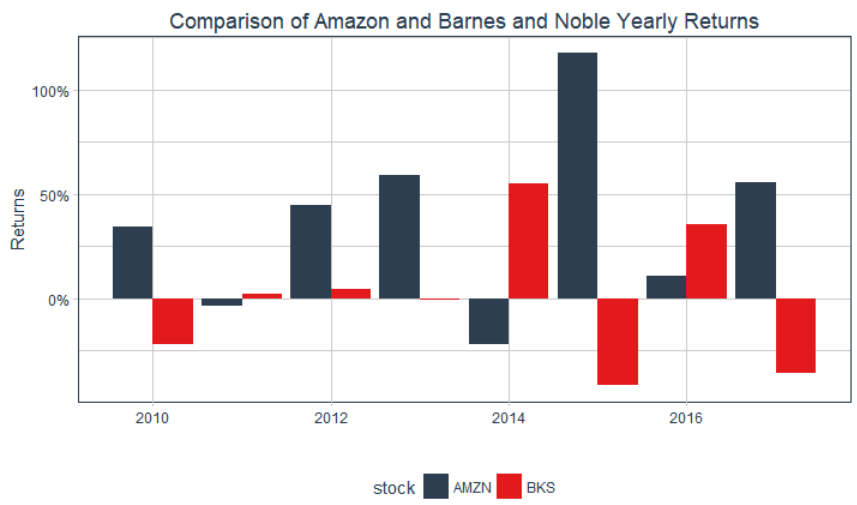
\includegraphics[scale=0.75]{PS6a_Nash}
\caption{Amazon vs. Barnes and Noble Returns}
\label{fig:PS6a_Nash}
\end{figure}

This figure shows that Amazon stock returns have generally been much better than Barnes and Noble returns since 2015, except in 2011 and 2014. I expected more of an inverse relationship between the two than I found.


\section{Second Visualization}

I selected the second dataset from Kaggle, which I used to show the relationship between age and heroin use. I wanted to show the relationship between age and any kind of drug use by adding up the columns of drug use, but the Hackathon took up the time I would've had to clean the data this weekend, so you can see in my script that I was unsuccessful in doing that. So, my visualization just expresses the relationship between heroin use and age. Note that "26029" denotes the age range "26-29." R is funky with hyphens, so I replaced it with zero instead of an underscore for a reason that I can't remember. I would've fixed that, but again, #Hackathon.

\begin{figure}[h!]
\centering
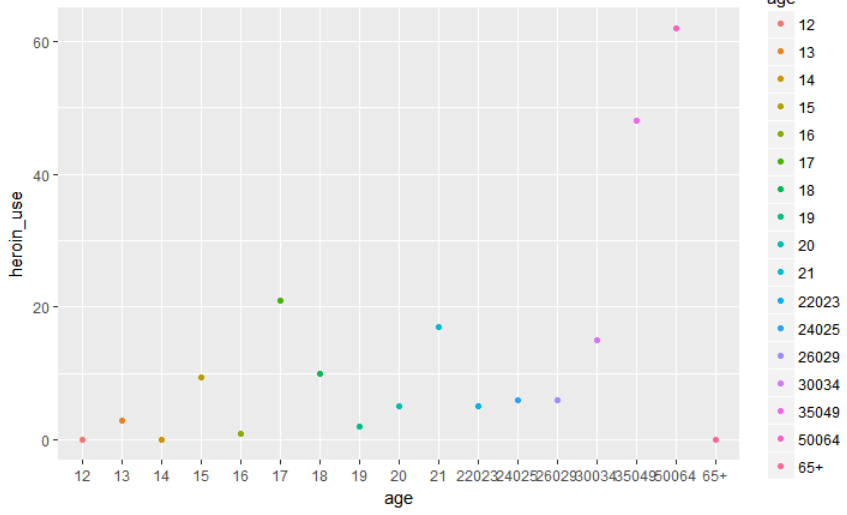
\includegraphics[scale=0.75]{PS6b_Nash}
\caption{Age and Heroin Use}
\label{fig:PS6b_Nash}
\end{figure}

This figure shows that heroin use increases with age until the age of 17, at which point heroin use declines. But, note a spike around age 21. I suspect that this is because of the complementary relationship between heroin and alcohol use. Or, let's be honest, most people drink before the age of 21, so maybe the difference is really that people can start hanging out at bars at age 21, and heroin dealers can find clients at bars. Finally, notice how weirdly high heroin usage is for 40-year-olds. Midlife crisis...?


\section{Third Visualization}

The last dataset was already cleaned by yours truly for a project I did two years ago. I was trying to show that the GRI (a metric by Pew that quanitifies how much a government restricts religious practice) increases in countries that experience high levels of immigration. For this visualization, however, I just looked at the relationships between unemployment and the GRI. This is because countries with higher unemployment usually experience more political unrest, religious institutions act as an organized channel through which political opposition becomes manifest, and, therefore, governments decide to suppress this by cracking down on the practice of religion. Back when I cleaned this data, I only knew how to use Excel and STATA, so I just ommitted all countries without a GRI measure (manually--LOL), then did mean imputation for any missing values in the dependent and control variables. You won't find that in my R script since the data was already cleaned and ready for visualization for my other project.

\begin{figure}[h!]
\centering
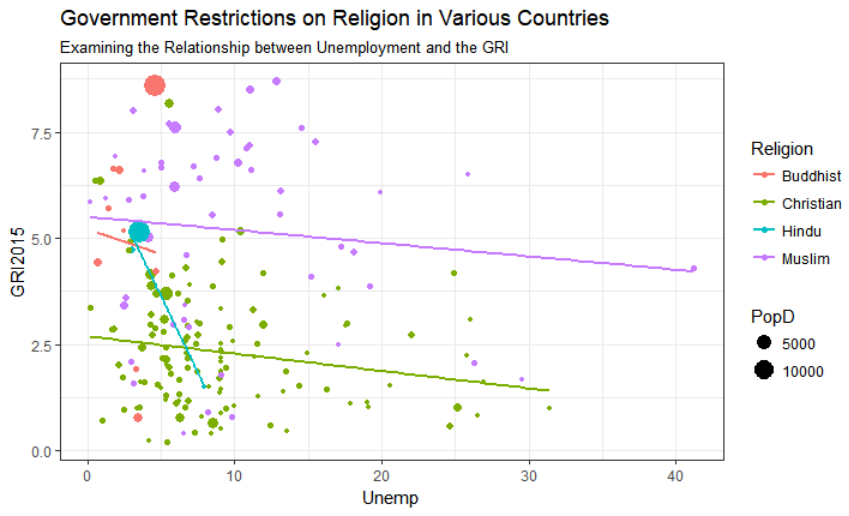
\includegraphics[scale=0.75]{PS6c_Nash}
\caption{Unemployment and the GRI}
\label{fig:PS6c_Nash}
\end{figure}

This figure shows that there really isn't too much of a relationship between unemployment and the GRI. Most countries seem to be around the same level of unemployment, and within that range, the GRI is pretty random. The color expresses the majority religion of the country. Note that Christian countries have generally lower GRIs, and Muslim countries have higher GRIs. Also, the size of the dot represents the population of the country in hundred thousands. Notice that the two most highly populated countries have comparatively high GRIs.


\end{document}